
\newcommand{\descripcion}{Gu\'ia de Estudio Bimestral, Primer Bimestre}
\newcommand{\grado}{Primero de secundaria}
\newcommand{\ciclo}{Ciclo escolar: 2015--2016}
\newcommand{\papel}{letterpaper} %letterpaper, legalpaper ...
\newcommand{\fecha}{5 de octubre de 2015}
\author{Ing. Arturo Canedo \\ M. en C. Reinaldo Zapata}
% \author{M. en C. Reinaldo Zapata}

\documentclass[11pt]{article}
\usepackage[\papel]{geometry}
\usepackage{enumitem}

% \title{\flushleft \seccion \\ \descripcion \\  \grado \\ \ciclo}

% \newcommand\BackgroundLogo{
% \put(162,365){
% \parbox[b][\paperheight]{\paperwidth}{%
% \vfill% \centering
% \includegraphics[width=5cm,height=2.5cm,keepaspectratio]{/Users/reinaldo/Documents/clases/jassa/logo}%
% \vfill
% }}}



\title{\seccion \\ \descripcion \\  \grado \\ \ciclo}

\newcommand\BackgroundLogo{
\put(162,335){
\parbox[b][\paperheight]{\paperwidth}{%
\vfill
\centering
\includegraphics[width=5cm,height=2.5cm,keepaspectratio]{/Users/reinaldo/Documents/clases/jassa/logo}%
\vfill
}}}

\hyphenation{con-ti-nua-ción}

\usepackage{enumitem}
\usepackage[T1]{fontenc} %fuentes
\usepackage{lmodern} %fuente mejorada
\usepackage[spanish]{babel}
\decimalpoint
\usepackage{fullpage}
\usepackage{multicol}
\usepackage{graphicx}
\usepackage{eso-pic}
\usepackage{multirow}
\usepackage{subfigure}


%Modificación del formato de las ecuaciones y el numerado de las mismas
\usepackage[leqno,fleqn]{amsmath}
\makeatletter
  \def\tagform@#1{\maketag@@@{#1\@@italiccorr}}
\makeatother
\renewcommand{\theequation}{\fbox{\textbf{\arabic{equation}}}}


\begin{document}
\AddToShipoutPicture*{\BackgroundLogo}
\ClearShipoutPicture
\date{\fecha}
\maketitle
% \thispagestyle{empty}


Nombre del alumno:\,\line(1,0){244}\,.\hspace*{.2cm} No. de lista:\,\line(1,0){35}\,.

\grado, grupo:\,\line(1,0){30}\,.

\vspace{5mm}

El prop\'osito de esta gu\'ia de estudio es proporcionar al alumno un repaso de
los temas que ser\'an vistos en el examen bimestral. Contesta de forma correcta,
en hojas de cuadro grande, cada uno de los reactivos que se muestran a
continuaci\'on.

\section{Fracciones y decimales}

Convierte cada fracci\'on a decimal y viceversa. Simplifica tus resultados si es
posible.

\begin{multicols}{4}

\begin{equation}    \frac{3}{4} =    \end{equation}

\begin{equation}    \frac{15}{64} =  \end{equation}

\begin{equation}    \frac{21}{25} =  \end{equation}

\begin{equation}    0.23 =          \end{equation}

\begin{equation}    0.049 =         \end{equation}

\begin{equation}    9.275 =         \end{equation}

\begin{equation}    4\frac{5}{16} =  \end{equation}

\begin{equation}    \frac{14}{75} =  \end{equation}

\begin{equation}    \frac{17}{100} = \end{equation}

\begin{equation}    0.875 =         \end{equation}

\begin{equation}    3.75 =          \end{equation}

\begin{equation}    3.1416 =        \end{equation}

\end{multicols}


\newpage

Completa la siguiente tabla.

\vspace {0.5cm}

\begin{center}
\begin{tabular}{|c|c|c|}
\hline
\hline
Cantidad & Cantidad con letra & N\'umero decimal \\
\hline
\hline
$3\frac{2}{5} $ && \\
\hline
$2\frac{1}{4} $ && \\
\hline
& Seis enteros tres quintos & \\
\hline
&& 2.7\\
\hline
\hline
\end{tabular}
\end{center}

\vspace{1cm}

\section{Recta num\'erica}

Traza una recta num\'erica de 12 cuadros de longitud. Coloca en el extremo
izquierdo el n\'umero cero (0) y en el extremo derecho el n\'umero dos (2).
Usando esa misma recta ubica las siguientes cantidades: \hspace{5mm}
\begin{multicols}{5}
\begin{enumerate}[label=\alph*)] \itemsep-.3em
\item $\displaystyle\frac{4}{5} $ \hspace{5mm} 
\item 0.9 \hspace{5mm} 
\item 0.6 \hspace{5mm} 
\item 1.1 \hspace{5mm}
\item $\displaystyle\frac{11}{6} $
\end{enumerate}
\end{multicols}

\vspace{1cm}

Traza una recta num\'erica de 20 cuadros de longitud. Coloca en el extremo
izquierdo el n\'umero cero (0) y en el extremo derecho el n\'umero cuatro (4).
Usando \'esta ubica las siguientes cantidades: \hspace{5mm}
\begin{multicols}{4}
\begin{enumerate}[label=\alph*)] 
\item 0.5  

\item $\displaystyle\frac{4}{3} $  

\item 2.25  

\item $\displaystyle\frac{33}{4} $ 

\item 1.2  

\item $\displaystyle\frac{12}{5} $  

\item $\displaystyle\frac{13}{5} $  

\item 3.8  

\item $\displaystyle\frac{17}{7} $  

\item 2.125  

\item $\displaystyle\frac{7}{8} $  

\item 0.6  

\end{enumerate}
\end{multicols}

\vspace{1cm}

\section{Comparaci\'on de n\'umeros}

Compara los n\'umeros fraccionarios y decimales; utiliza los s\'imbolos mayor que
(>), menor que (<) e igual (=), seg\'un sea el caso
\begin{multicols}{3}
\setcounter{equation}{0}

\begin{equation} 0.42 \quad \line(1,0){35} \quad 0.4    \end{equation}

\begin{equation} \frac{1}{3} \quad \line(1,0){35} \quad 0.3   \end{equation}

\begin{equation} 0.56 \quad \line(1,0){35} \quad \frac{1}{2}   \end{equation}

\begin{equation} 3.7 \quad \line(1,0){35} \quad 3.701   \end{equation}

\begin{equation} \frac{1}{6} \quad \line(1,0){35} \quad 0.7   \end{equation}

\begin{equation} 4.7 \quad \line(1,0){35} \quad  4.710  \end{equation}
\end{multicols}

\vspace{1cm}

\section{problemas}

A una botella de aceite comestible de $\frac{3}{4}$ de litro se le
extrae $\frac{1}{5}$ de litro para preparar cierto platillo. ?`Qu\'e fracci\'on 
de litro queda en la botella de aceite?

\vspace{1cm}

Un pescador vendi\'o $\frac{1}{6}$ del total de su pesca, $\frac{1}{3}$ 
de la misma la entreg\'o en el mercado, guard\'o $\frac{1}{4}$ para su familia y
el resto lo don\'o a un albergue. ?`Qu\'e fracci\'on de la pesca don\'o?

\vspace{1cm}

En cierto trabajo a los empleados les es otorgado un tiempo de
descanso de $1\frac{1}{2}$ horas durante su jornada laboral. Cierta trabajadora
utiliz\'o $\frac{3}{4}$ de hora comiendo, $\frac{1}{2}$ de hora caminando y
$\frac{1}{6}$ viajando en autob\'us para llegar de regreso a su trabajo.
Despu\'es todo \'esto, ?`Le sobr\'o o le falt\'o tiempo? ?`Cu\'anto tiempo le
sobr\'o o le falt\'o?

\vspace{1cm}

Orlando desea saber que calificaci\'on obtuvo en cada una de sus
asignaturas. Para hacerlo debe completar la tabla. Analiza y completa la tabla:

\vspace{1cm}

\begin{center}
\begin{tabular}{|l|c|c|c|c|c|}
\hline
\hline
Asignatura & Aceirtos  & Total de  & Fracci\'on & Calificaci\'on & Calificaci\'on \\
           & obtenidos & reactivos &            &                & base 10 \\
\hline
\hline
Espa\~nol & 86 & 100 & $\displaystyle\frac{86}{100}$ & 0.86 & 8.6 \\ 
\hline
Matem\'aticas & 32 & 65 &&&\\
\hline
Biolog\'ia & 25 & 30 &&&\\
\hline
Historia & 65 & 100 && 0.65 & \\
\hline
Asignatura estatal & 42 & 95 &&&\\ 
\hline 
\hline 
\end{tabular}
\end{center}


\vspace{1cm}

En una bolsa hay un total de 30 canicas de las cuales cinco (5) son de
color amarillo, diez (10) son de color verde y el resto azules. Responde a las
siguientes preguntas:

\begin{enumerate}[label=\alph*)] \itemsep-.3em
\item ?`Qu\'e fracci\'on del total representan las canicas azules?
\item ?`Qu\'e fracci\'in decimal represntan las canicas amarillas?
\item ?`Qu\'e decimal representan las las canicas azules?
\item que decimal represntan las canicas verdes y azules juntas?
\end{enumerate}

\vspace{1cm}

\section{Geometr\'ia}

Busca en el diccionario la definici\'on de las siguientes palabras. 

\vspace{5mm}

Arista:

\vspace{1.5cm}

Per\'imetro:

\vspace{2cm}


Ahora explica con tus palabras las definiciones que apuntaste en el inciso
anterior.

\vspace{4cm}


Calcula el per\'imetro de las figuras que se muestran a continuaci\'on usando
los datos que se muestran en cada una de ellas.

\begin{minipage}[t]{0.3\linewidth}

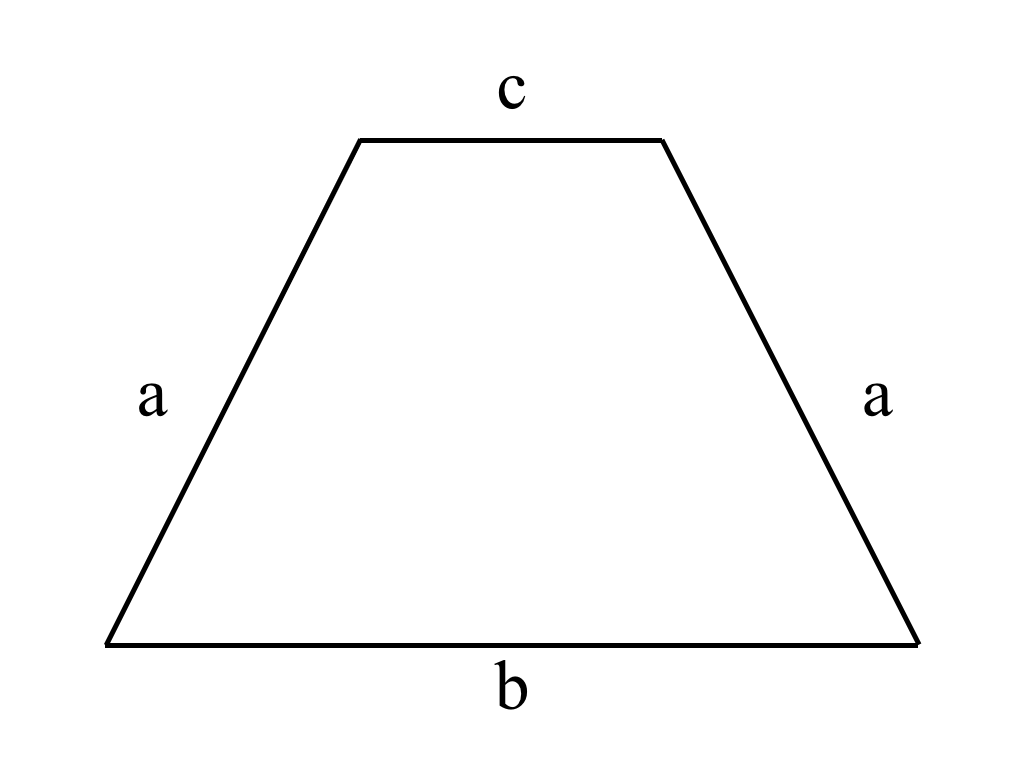
\includegraphics[width=0.9\linewidth]{figures/figures001.png}

a=4\,cm

b=6\,cm

c=2\,cm

\vspace{5mm}

F\'ormula:

\vspace{2cm}

Per\'imetro:

\end{minipage}
\begin{minipage}[t]{0.3\linewidth}

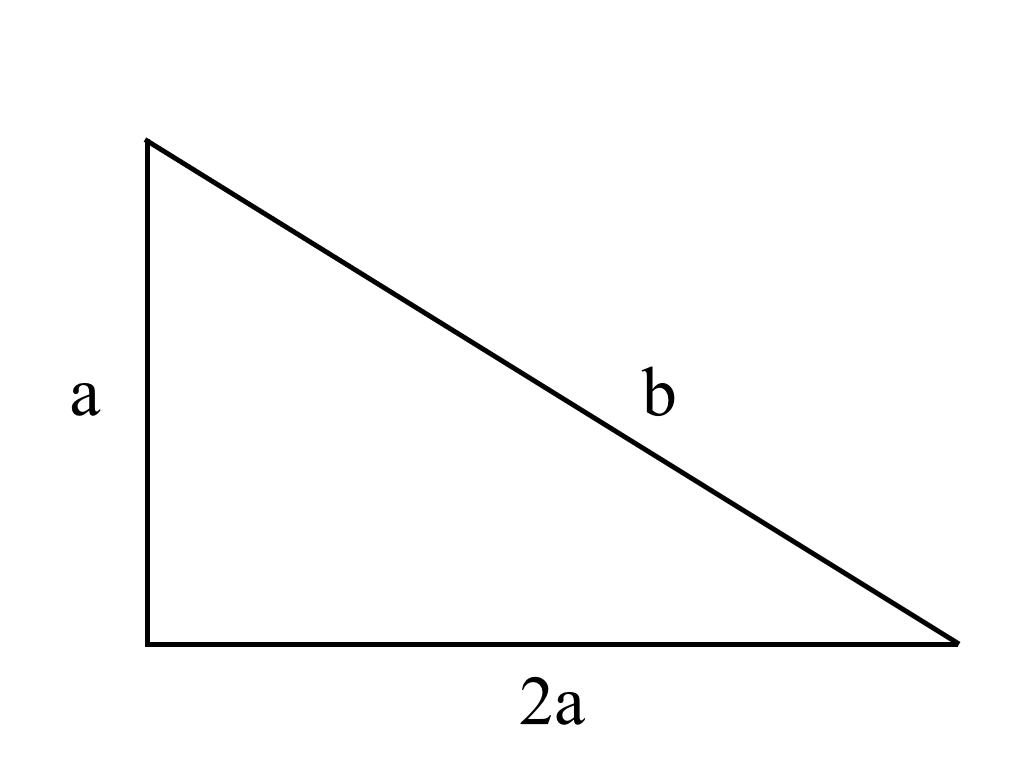
\includegraphics[width=0.9\linewidth]{figures/figures002.png}

a=5\,cm

b=10\,cm

\vspace{10mm}

F\'ormula:

\vspace{2cm}

Per\'imetro:

\end{minipage}
\begin{minipage}[t]{0.3\linewidth}

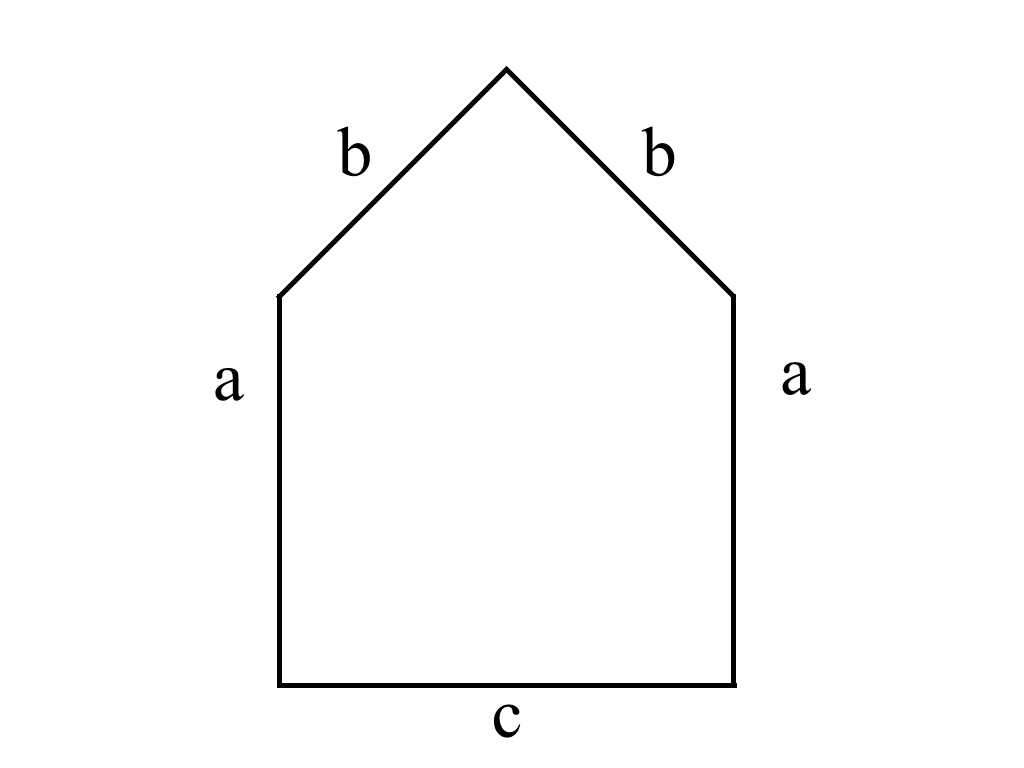
\includegraphics[width=0.9\linewidth]{figures/figures003.png}

a=15\,cm

b=6\,cm

c=8\,cm

\vspace{5mm}

F\'ormula:

\vspace{2cm}

Per\'imetro:

\end{minipage}

\newpage

\section{Sucesiones y series}

Observa las figuras que se muestran a continuaci\'on y responde las preguntas.

\begin{figure}[h]
    \centering
    
\includegraphics[width=0.17\linewidth]{figures/figures004.png}
    
\includegraphics[width=0.17\linewidth]{figures/figures005.png}
    
\includegraphics[width=0.17\linewidth]{figures/figures006.png}\\
    1 \hspace{2.5cm} 2 \hspace{2.5cm} 3
\end{figure}

?`Cu\'antos elementos tiene cada figura?

?`Cu\'antos elementos tendr\'a la siguiente figura?

?`Cu\'antos puntos habr\'a en las figuras 6 y 7?

\vspace{1cm}

Imagina que las aristas de los cuadrados de las siguientes figuras est\'an
formados por palillos. 

\begin{figure}[h]
    \centering
    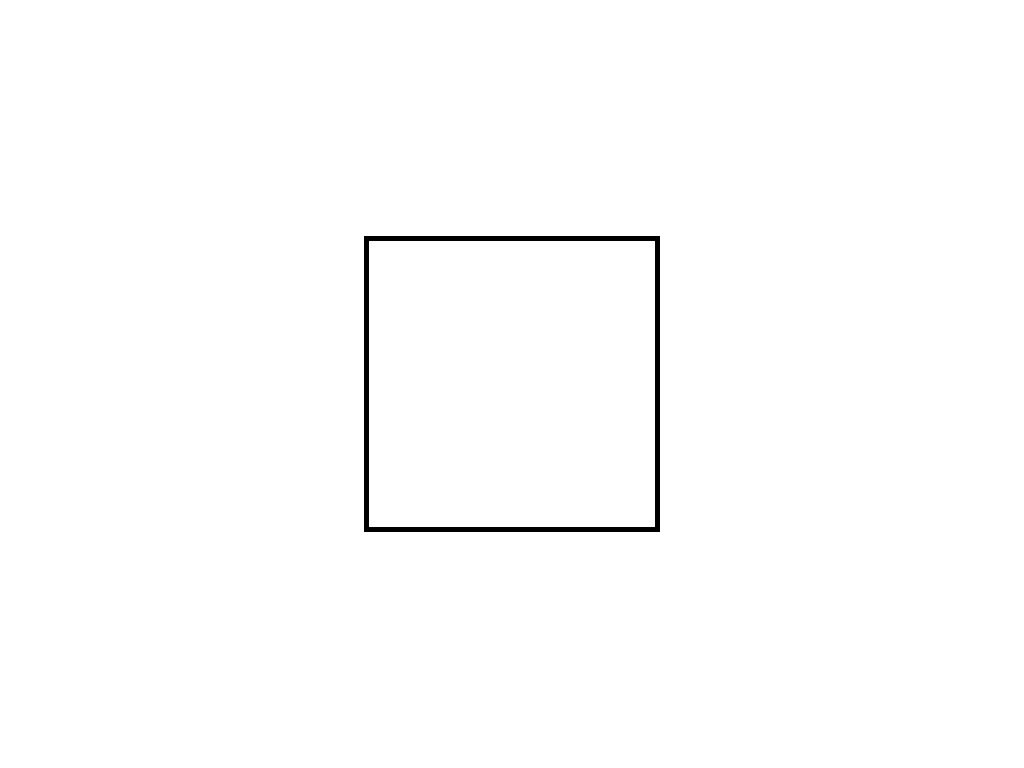
\includegraphics[width=0.2\linewidth]{figures/figures007.png}
    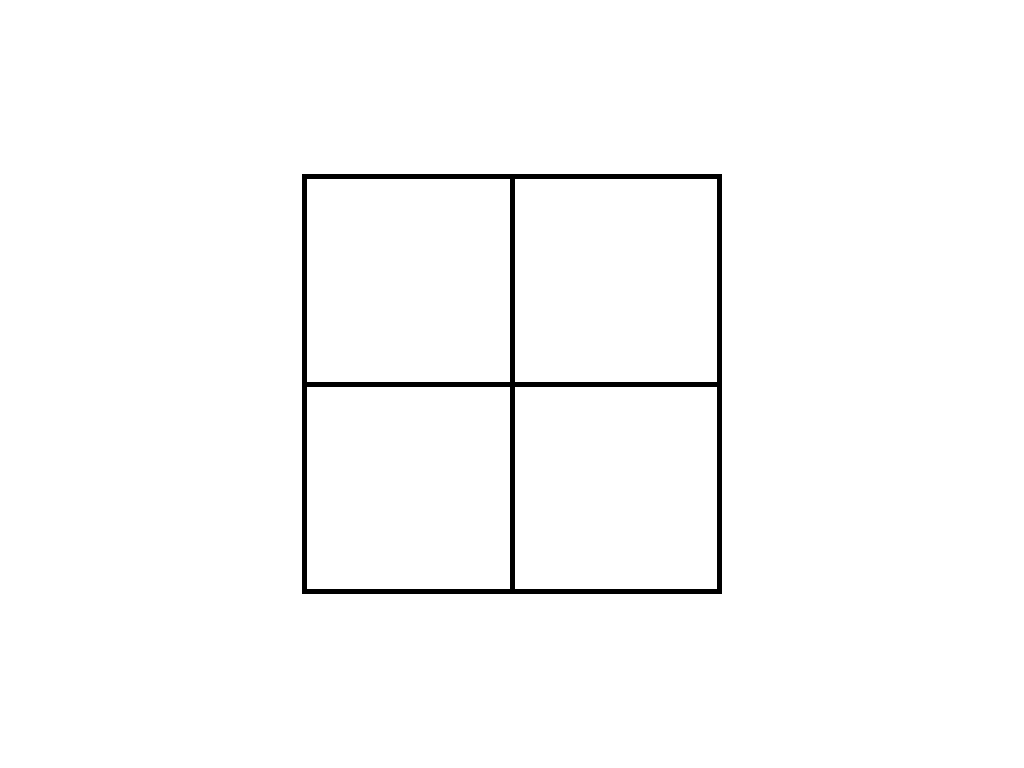
\includegraphics[width=0.2\linewidth]{figures/figures008.png}
    
\includegraphics[width=0.2\linewidth]{figures/figures009.png}\\
    1 \hspace{3cm} 2 \hspace{3cm} 3
\end{figure}

?`Cu\'antos palillos se necesitan para construir la figura 4?

?`Y la figura 5?

?`Y para la figura 10?

Completa la siguiente tabla:

\begin{center}
\begin{tabular}{|l|c|c|c|c|c|c|c|c|}
\hline
Figura &\hspace{5mm}1\hspace{5mm} & \hspace{5mm}2\hspace{5mm} & \hspace{5mm}3\hspace{5mm} & \hspace{5mm}4\hspace{5mm} & \hspace{5mm}5\hspace{5mm} & \hspace{5mm}6\hspace{5mm} & \hspace{5mm}7\hspace{5mm} & \hspace{5mm}8\hspace{5mm}   \\
\hline
\hline
No. de palillos & 4 & 12 & 24 & &&&&\\ 
\hline
\end{tabular}
\end{center}

\section{Jerarqu\'ia de las operaciones}

Acomoda los siguientes incisos de la izquierda en
las l\'ineas que est\'an a la derecha acorde al orden en que se tienen que
realizar las operaciones.

\vspace{1cm}

\begin{minipage}[t]{0.5\textwidth}
Multplicaci\'on y divisi\'on.

Potencias y ra\'ices: $r^{2}$, $4^{2}$, $\sqrt{2}$, $\sqrt{25}$.

Suma y resta.

Signos de agrupaci\'on: (), [], \{\}.

\end{minipage}
\begin{minipage}[t]{0.5\textwidth}

1.-\,\line(1,0){200}\,.

\vspace{3mm}

2.-\,\line(1,0){200}\,.

\vspace{3mm}

3.-\,\line(1,0){200}\,.

\vspace{3mm}

4.-\,\line(1,0){200}\,.

\vspace{3mm}

\end{minipage}

\newpage

Determina si el resultado de las siguientes operaciones con fracciones es
correcto o incorrecto resolviendo cada iciso.

\setcounter{equation}{0}

\begin{equation}
\left( \frac{1}{3} + \frac{2}{30} \right) \div \frac{1}{6} = 2\frac{2}{5}
\end{equation}

\begin{equation}
\frac{3}{5} \div \left( \frac{2}{3} + \frac{5}{6} \right) = \frac{2}{5}
\end{equation}

\begin{equation}
\left( 1 - \frac{1}{3} \right) \div \left( 1 - \frac{1}{5} \right) = \frac{4}{6}
\end{equation}



\end{document}























